\chapter{Metodología }
\section{Formulas junto a texto}
\textbf{Cuadrado de un binomio}. Sea. $(a+b)^{2} = (a+b)(a+b)$ donde $a$ y $b$ representan números algebraicos cualesquiera, positivos o negativos. Por lo tanto $ (a+b)^{2} + 2ab + b^{2}$

\section{Formulas independiente}
\textbf{Cuadrado de un binomio}
\[
  (a+b)^{2} = (a+b)(a+b)
\]
 donde $a$ y $b$ representan números
\[
 (a+b)^{2} + 2ab + b^{2}
 \]
 
\begin{equation}
 (a+b)^{2} + 2ab + b^{2}
\end{equation}
\begin{equation}
 (a+b)^{2} + 2ab + b^{2}
\end{equation}

\section{Alineacion de ecuaciones con el comando align}

\begin{align}
 x &= 3a + b\\
 x &= a + b\\
 x &= a + 5b
\end{align}

\newpage

\section{Fracciones}
\begin{itemize}
\item Junto a texto $\dfrac{x}{y}$
\item Junto a texto $\frac{x}{y}$
\end{itemize}

\section{Paquete Graphicx}
\begin{center}

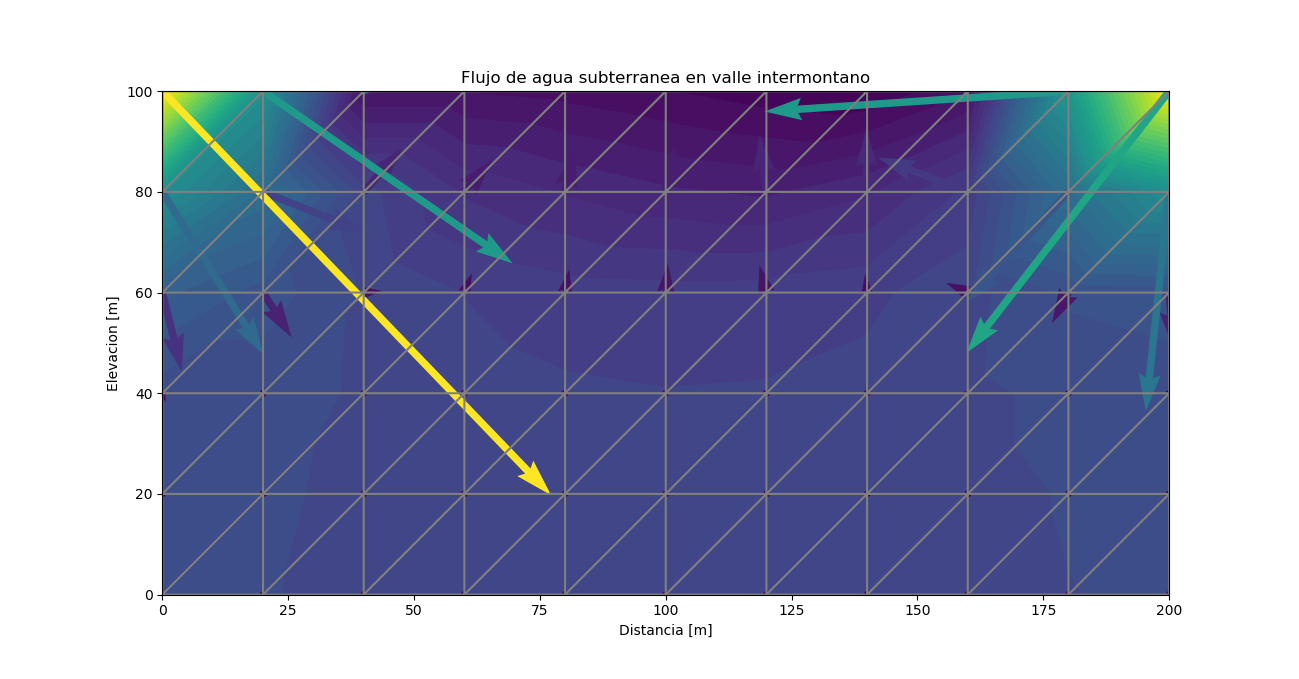
\includegraphics[scale=0.5]{Figure_2.png}

\end{center}

\section{Objetos flotantes}

\begin{figure}[!ht]
\centering 
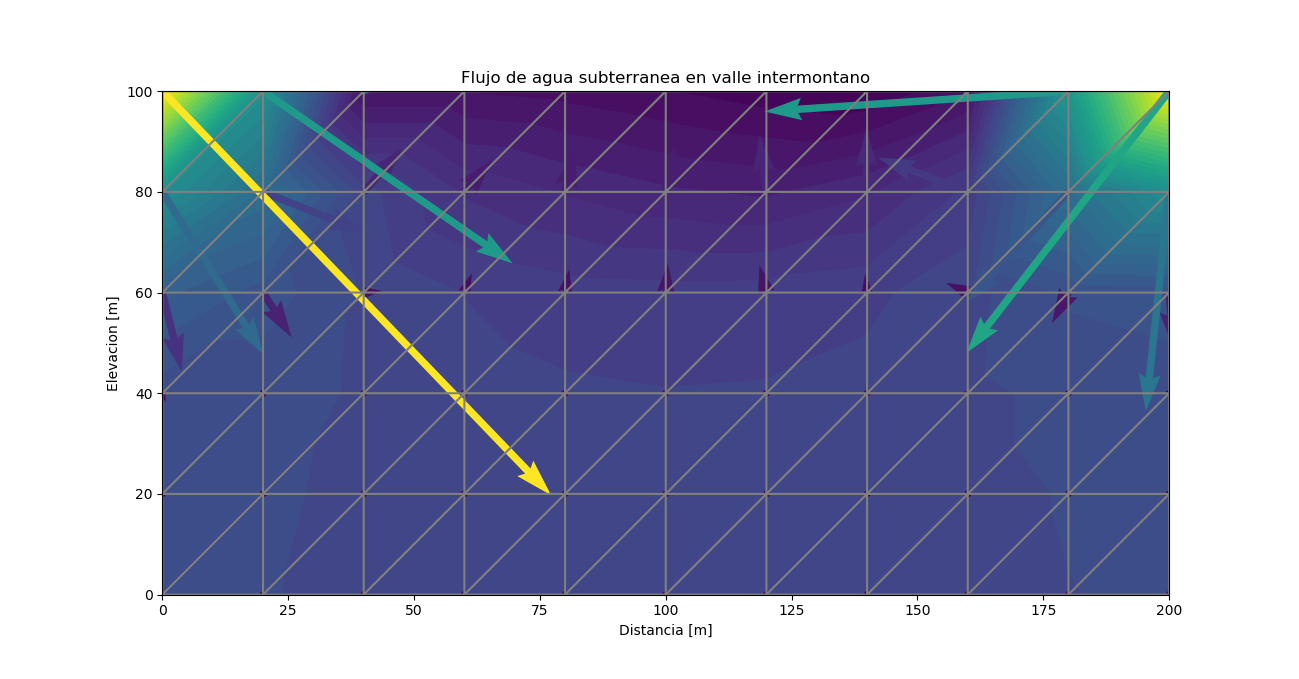
\includegraphics[scale=0.5]{Figure_2.png}
\caption{imagen a escala 0.5}
\label{figura1}
\end{figure}
